% intensity
% spectral distribution
% solar geometry
% saules stāvoklis debesīs
% un virziens, kurā stara starojums krīt uz dažādu virzienu un ēnojuma virsmām


% Definīcijas
% Saules plankums - magnētiskās plūsmas koncentrācija bipolāros klāsteros vai grupās, kas novērojama kā tumšs plankums uz Saules fotosfēras.\\
% Saules plankumu cikls - aptuveni 11 gadus ilga kvaziperiodiska variācija saules plankuma skaitlī. Magnētiskā lauka polaritātes modelis mainās ar katru ciklu.\\
% Saules plankuma skaitlis - Dienas saules plankuma aktivitātes indekss (R), definēts kā R = k(10g + s), kur
% s - individuālo plankumu skaits;
% g - saules plankumu grupu skaits;
% k - observatorijas faktors.
% total solar irradiance (TSI) - Solar energy per unit time over a unit area perpendicular to the Sun’s rays at the top of Earth’s atmosphere.
% \\http://lasp.colorado.edu/home/sorce/reference/glossary/

\section{Saules apstarojums}

Lielākā daļa Saules emitētās enerģijas tiek saražota kodolreakcijās fotosfērā.

Saņemto enerģiju laika vienībā uz uz laukuma vienības perpendikulāri starojuma izplatīšanās virzienam 1 AU attālumā integrēta pa visiem viļņu garumiem raksturo solārā konstante ($G_{sc}$).



Solārā konstante $G_{sc}$ ir saņemtā enerģija laika vienībā uz laukuma vienības perpendikulāri starojuma izplatīšanās virzienam 1 AU attālumā integrēta pa visiem viļņu garumiem.\cite{ThermalProcesses}


Kaut gan absolūtais kopējais saules apstarojuma vērtība ir kontroversiāla, jo laika gaitā mērīta ar dažādiem radiometriem un kosmosa misijām, piemēram, 
iegūtas dažādas vērtības,

tas tiek risināts veidojot salikumus (composites) no dažādu misiju datu apkopojuma.

apkopojot dažādu (ne vienmēr pārklājušos) misiju novērojumus



Daudzi novērošanas ieraksti lielā mērā balstās uz spēju apvienot dažādus (ne vienmēr pārklājošos) novērojumus vienā salikumā.

dažādu tikai daļēji pārklātu viena fiziskā novērojuma 
gadījumu apvienošana vienā salikumā


Dažādu (un tikai daļēji pārklātu) viena un tā paša fiziskā daudzuma laikrindu apvienošana vienā kompaktā ir gan zinātnisks, gan statistisks izaicinājums, kas rodas daudzos kontekstos, jo īpaši paleoclimaticreconstructions



Par labāko saules apstarojuma reprezentāciju tiek uzskatīti TIM mērījumi, uz kuriem tiek balstīts šis darbs.


korelē ar sunspot number



\begin{table}[h]
    \caption{TSI mērījumu vēsture} % caption iet pirms tabulas
    \begin{center}
    \begin{tabular}{| r | c | l |}
    \hline
    radiometrs & misija & darbības laiks \\ \hline
    Hickey-Frieden & NIMBUS-7 & 1978--1992  \\ \hline
	ACRIM I & Solārā Maksimuma Misija (SMM) & 1980--1989 \\ \hline
	ACRIM  & Zemes Radiācijas Budžeta Satelīts (ERBS) & 1984--2003 \\ \hline
	ACRIM II & Augšējās Atmosfēras Izpētes Satelīts (UARS) & 1991--2001 \\ \hline
	VIRGO & Solārā un Heliosfēras observatorija (SOHO)& 1996--pašlaik \\ \hline
	ACRIM III & ACRIMSAT  & 2000--pašlaik \\ \hline
	TIM & Saules Radiācijas un Klimata Eksperiments (SORCE) & 2003--pašlaik\\ \hline
    \end{tabular}
    \end{center}
    \label{tab:radiometers}
\end{table}


Kopējais saules apstarojums (TSI) ir saules starojuma absolūtās intensitātes mērījums integrēts visā saules enerģijas diskā un visā saules enerģijas spektrā.

diennakts vidējais apstarojums 1 AU attālumā no Saules.

Norāda uz solārās radiācijas izmaiņām, kas ietekmē solārās enerģijas apjomu uz Zemes atmosfēras augšējiem slāņiem.


Šajā darbā tiek izmantot TSI dati no SORCE (SOlar Radiation and Climate Experiment) TIM (Total Irradiance Montior) dati, pēc kuriem absolūtā vērtība ir $1360.8 \pm 0.5 \textrm{Wm}^{-2}$, jo tie ir precīzākie un ...\cite{Frohlich2012}

\begin{figure}[h]
    \centering
    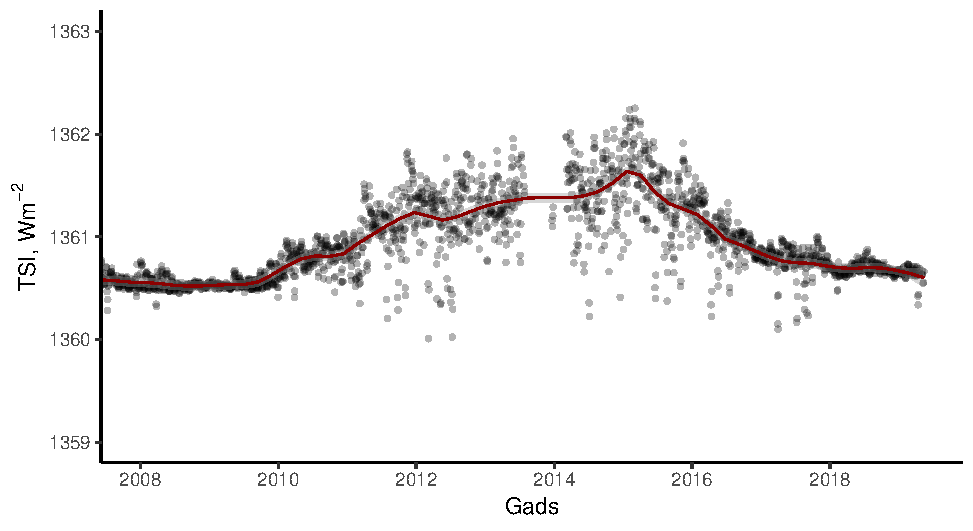
\includegraphics[width=\linewidth]{figures/misc/TSI_8-19.pdf}
    \caption{Kopējais saules apstarojums 24. saules ciklā \cite{TSIdata}}
    \label{fig:TSI1}
\end{figure}

\begin{figure}[h]
    \centering
    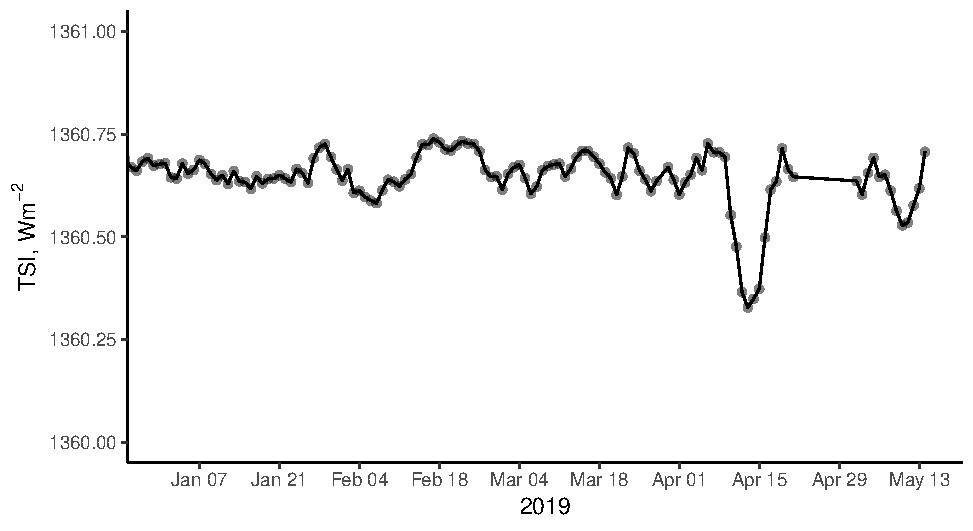
\includegraphics[width=\linewidth]{figures/misc/TSI.pdf}
    \caption{Kopējais saules apstarojums solāro paneļu datu ieguves laikā \cite{TSIdata}}
    \label{fig:TSI2}
\end{figure}

\begin{figure}[h]
    \centering
    \includegraphics[width=\linewidth]{figures/misc/LV_DNI.png}
    \caption{Tiešais normālais apstarojums \cite{solargis}}
    \label{fig:lv_DNI}
\end{figure}
\begin{figure}[h]
    \centering
    \includegraphics[width=\linewidth]{figures/misc/LV_GHI.png}
    \caption{Globālais horizontālais apstarojums Latvijā \cite{solargis}}
    \label{fig:lv_GHI}
\end{figure}
\begin{figure}[h]
    \centering
    \includegraphics[width=\linewidth]{figures/misc/LV_PVOUT.png}
    \caption{PV potenciālā jauda \cite{solargis}}
    \label{fig:lv_PVOUT}
\end{figure}
